
\documentclass[10pt,letterpaper]{article}
\usepackage{cogsci}
\usepackage{apacite}
\renewcommand\bibliographytypesize{\small}
\usepackage[english]{babel}
\usepackage[utf8x]{inputenc}

\usepackage{color,soul}
\usepackage{amsmath}
\usepackage{graphicx}


\usepackage{graphicx, subcaption}
\usepackage[section]{placeins}
\usepackage{subcaption}
\usepackage{pslatex}


\cogscifinalcopy % Uncomment this line for the final submission 

\newcommand{\tg}[1]{\textcolor{blue}{#1}}
\newcommand{\gk}[1]{\textcolor{red}{#1}}

\title{Exploring informal science interventions to promote children's understanding of natural categories}
\author{George Kachergis$^1$, Todd M. Gureckis$^2$, Marjorie Rhodes$^2$ \\
     $^1$Department of Psychology, Stanford University, Palo Alto, CA \\
     $^2$Department of Psychology, New York University, New York, NY \\
  }

\begin{document}
\maketitle

\begin{abstract}
Categories carve up the world in a structured way, allowing people to inductively reason about the properties of novel exemplars. 
Children are still in the process of learning category structure, and often fail to leverage the inductive power of these representations to their advantage.
For example, young children generally fail to recognize the value of sampling diverse exemplars to support category-wide generalization.
This study investigates whether teaching children the structure within a natural category increases diversity-based inductive reasoning.
In an informal science learning environment, we presented 259 children aged 5 to 8 years with exemplars of the three main types of birds: raptors, songbirds, and waterbirds.
After a short dialogue pointing out the various within-type similarities and between-type differences, children's diversity-based inductive reasoning did not significantly improve, despite them evidencing a better understanding of the category's structure. 
Instead, children tended to avoid sampling waterbirds, the least typical cluster of birds. 
These patterns suggest that children's neglect of sample diversity is unlikely to be solely due to their relative ignorance of category structure.


\textbf{Keywords:} 
category induction; diversity-based reasoning; category learning; 
\end{abstract}

\section{Introduction} 

Categories give us a way out of the infant's problem of ``feel[ing] it all as one great blooming, buzzing confusion'' \cite{James:1890}, allowing us to carve our sensations of the world into classes that are distinguished by relevant properties. 
By picking out shared features while ignoring superficial differences, categories enable us to learn inductively \cite{Rips:1975}, and allow us to reason about unseen properties. 
For example, having learned that one cat's fur is soft, we might generalize this to all cats, and proceed to seek out and pet all cats. 
Assuming that categories are homogeneous, in that the exemplars share many observable and unobservable features, offers further inductive power \cite{Gelman:1988}, but can also lead to serious errors: your house cat may be amenable to petting, but a cougar may not be. 
Learning how to account for such within-category variation while engaging in category-based inductive reasoning is a nontrivial problem for children.

There is considerable evidence that adults take within-category variability into account when evaluating the inductive power of evidence. 
For example, when making inferences about general properties of a category, adults view some samples of exemplars from a category as more informative than others \cite{Rips:1975,Osherson:1990}.
Sample diversity is one feature adults attend to when evaluating evidential strength, with more diverse samples (e.g., a lion and a house cat) being viewed as more informative than nondiverse samples (two house cats) \cite{Heit:2000}. 
Adults' preference for diverse samples indicates that they assume that observable variability across exemplars in a category is often correlated with variance in the hidden features, and it is thus informative to sample from diverse areas of the distribution. 

Adults find diverse samples more informative both when choosing evidence to sample \cite{Kim:2003,Lopez:1995,RhodesBrickman:2008,Rhodes:2008} and when rating the strength of inductive arguments \cite{Osherson:1990}.
In contrast, children below the age of nine often fail to consider sample diversity \cite{Gutheil:1997,Rhodes:2008,RhodesBrickman:2008}. 
For example, before age 9, children are equally likely to choose to examine an eagle and a robin as two robins to see whether all birds have a given property \cite{RhodesBrickman:2008,Rhodes:2008}. One reason why this might be the case is that young children often assume categories to be more homogeneous than adults do \cite{Gelman:2003}. For instance, preschool-aged children infer more readily than adults that a property seen in one exemplar is true for the whole category \cite{Rhodes:2008}.
Moreover, preschool-aged children believe that everyday categories identify an objective natural reality to a greater extent than adults do \cite{Kalish:1998}. Directly linking this tendency to assume that categories are homogeneous to diversity-based reasoning, 7-year-olds reliably chose diverse samples over nondiverse samples after they were primed with an example highlighting within-category variability \cite{Rhodes:2010}. 
This finding supports the idea that young children may default to a strong within-category homogeneity assumption, and also shows that they sometimes recognize the value of diverse samples when such an assumption is violated. 
Here, we test whether a more abstract variation prime--distinguishing structured clusters within a category--induces a preference for diversity-based reasoning. 

\subsection{The present study}
Imagine that you are trying to determine whether a novel, hidden property is true of all birds (e.g., ``Do all birds have \emph{scutella}?'').
Adults deem it better grounds for generalization to the entire category when two dissimilar birds (e.g., an eagle and a robin) are both found to have the hidden property, rather than two more similar birds (e.g., a robin and a swallow).
In the model proposed by \citeA{Osherson:1990}, the greater strength of the argument based on dissimilar birds is a result not of the similarity of the premise categories to the conclusion category, but of their similarity to the lowest-level category that covers both the premise and conclusion categories--that is, birds.
If on the other hand, one were asked to determine if all songbirds have \emph{scutella}, the robin and swallow premises would offer a better match to the inductive target, since the songbird cluster is the lowest-level category covering both the premises and the target.

The goal of this study is to teach children more about the heterogeneous structure of one natural category--birds--to determine whether that knowledge improves their inductive reasoning about that category.
Specifically, this study will teach young children (ages 5-8) that the bird category is clustered into songbirds, waterbirds, and raptors, and that birds within each cluster share many visible (e.g., talon and beak shape) and hidden properties. 
The didactic dialogue and displays (see Figures~\ref{fig:example_birds} and \ref{fig:display_cases}) used to teach the clusters will also highlight some of the variability within each cluster, and some cross-cluster similarities.
Our hypothesis is that teaching children the clustered structure of the bird category may encourage them to represent the category more heterogeneously (i.e., with clusters instead of a single prototype), and thus may improve their diversity-based inductive reasoning--both for induction to a cluster, and to the entire category of birds.
This study was conducted in the context of the American Museum of Natural History's Discovery Room with an interest in developing more effective exhibits.

\section{Experiment}

The purpose of the experiment is to investigate whether teaching children the clustered structure of a natural category (birds) improves their ability to do diversity-based inductive reasoning.
Specifically, after measuring children's knowledge of the bird category through pile sorting, we tested two interventions--display cases (e.g., Figure~\ref{fig:display_cases}) vs. poster-based (e.g., Figure~\ref{fig:example_birds}), presented along with a didactic dialogue meant to demonstrate that birds can be subcategorized into three clusters: raptors, songbirds, and waterbirds. 
The dialogue first highlights the variability of the category (e.g., ``Some are big, some are small; some have bright colors...'' and then defines the three main clusters, emphasizing correlated features and their causal relationships (e.g., ``Most water birds have webbed feet--see? That helps them swim.'')
After highlighting a few distinctive features for each cluster and naming four examples of birds in each, children were given a series of inductive sampling questions to generalize to either a given cluster, or to the entire bird category.
Finally, we again measured children's knowledge of birds by pile sorting.


\subsection{Methods}

\subsubsection{Participants}

Participants in this experiment were 265 children between the ages of 5 and 8 years old who were recruited at the American Museum of Natural History's Discovery Room. 
Of the 265 children recruited (per intervention: 99 in None, 94 in Exhibit, and 66 in Poster), we analyzed the data from 259 children (60 5-year-olds, 73 6-year-olds, 68 7-year-olds, and 58 8-year-olds) who completed the study.

\subsubsection{Stimuli}

This task was designed to fit thematically with the content of the AMNH Discovery Room activities, which emphasize the varying features between species of birds, among other animals. 
Eight diverse birds from each cluster were selected to be used as stimuli. Songbirds\footnote{Blue jays are not songbirds, so this cluster is more accurately described as passerines. Colloquially, all are songbirds.} included were the robin, swallow, starling, oriole, redwing blackbird, blue jay, sparrow, and cardinal. 
Raptors included were the barred owl, falcon, vulture, kestrel, barn owl, red-tailed hawk, bald eagle, and kite. 
Water birds included were the tern, mallard duck, puffin, sea gull, harlequin duck, flamingo, goose, and anhinga. 
For the intervention conditions, four birds from each cluster were selected to be shown either on a poster, shown in Figure~\ref{fig:example_birds}, or in display cases as in  Figure~\ref{fig:display_cases}. 
The same exemplars were used in both intervention conditions. For the sorting task, each of the 24 birds was printed in color on a single 8.5 x 11'' sheet of paper, with the size of each bird being according to their real-world scale. 
These birds appeared in different combinations during the sampling questions, as well.
All materials and the protocol are available online\footnote{http://github.com/diversity-based-reasoning-clusters}. 

\begin{figure}[h]
  \centering
  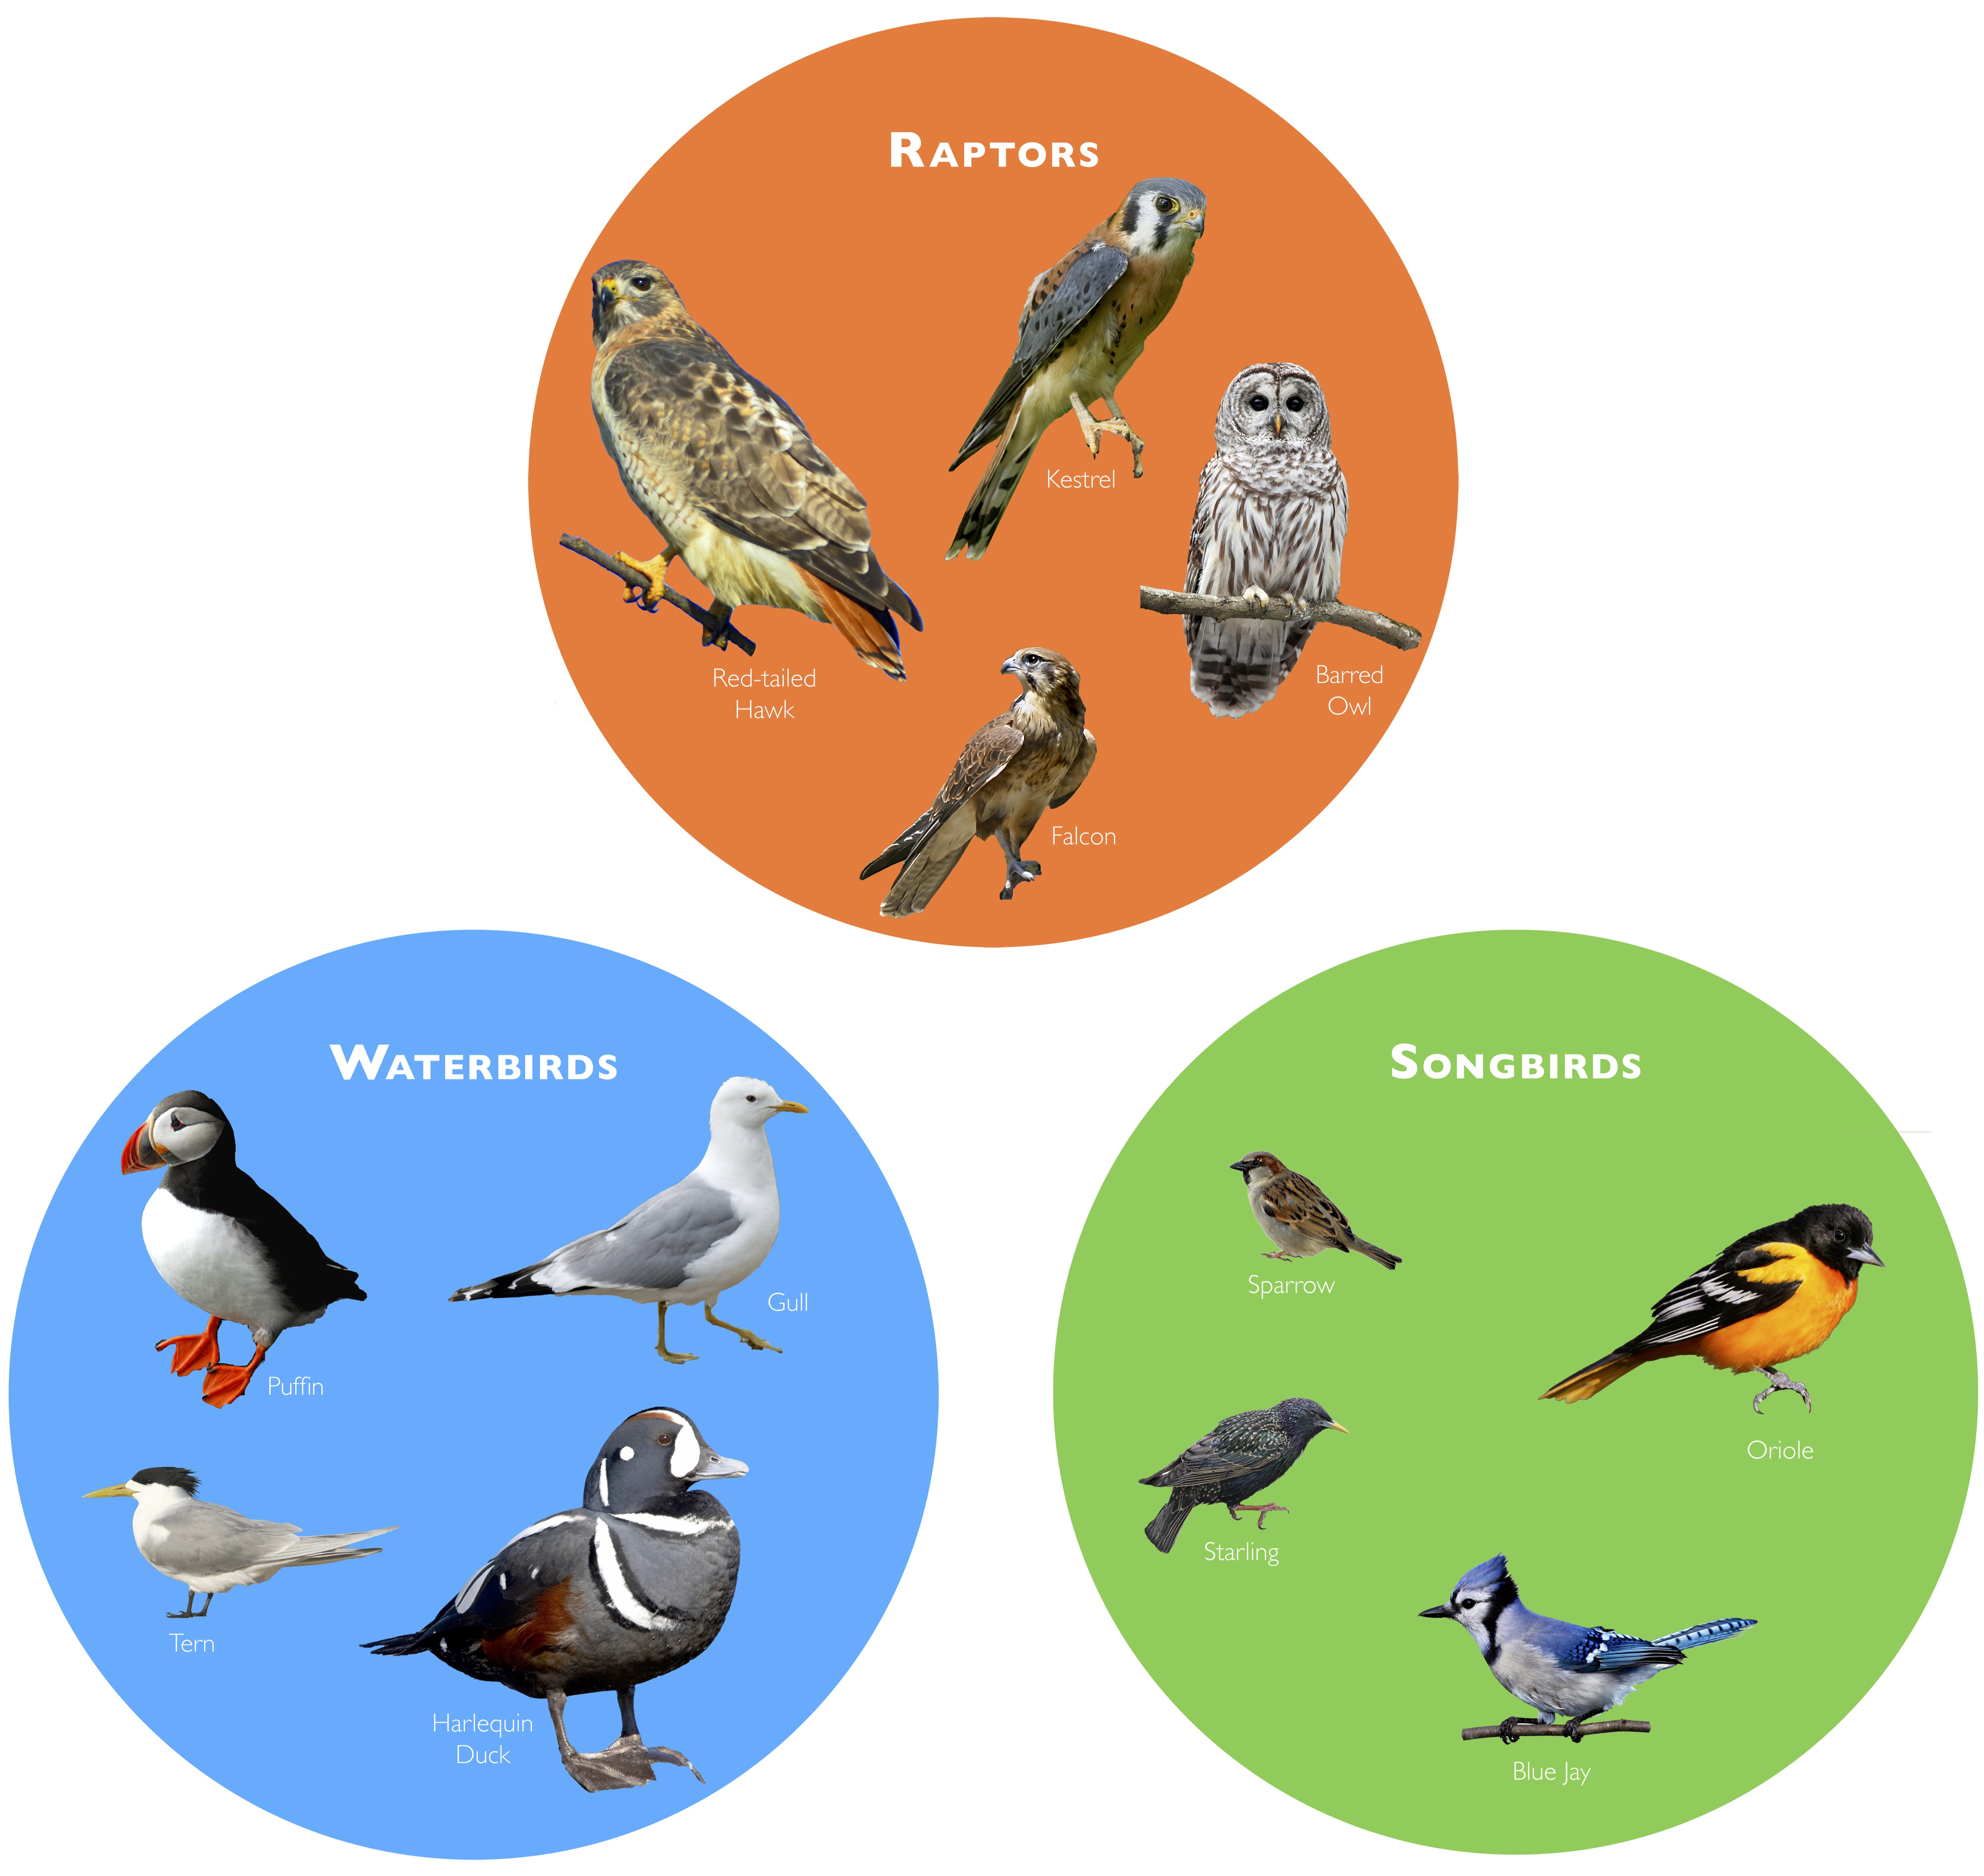
\includegraphics[width=0.48\textwidth]{figures/example_birds.png}
  \caption{The experiment used four birds from each cluster as stimuli. The poster intervention used this arrangement.} 
  \label{fig:example_birds}
\end{figure} 

\begin{figure}[h]
  \centering
  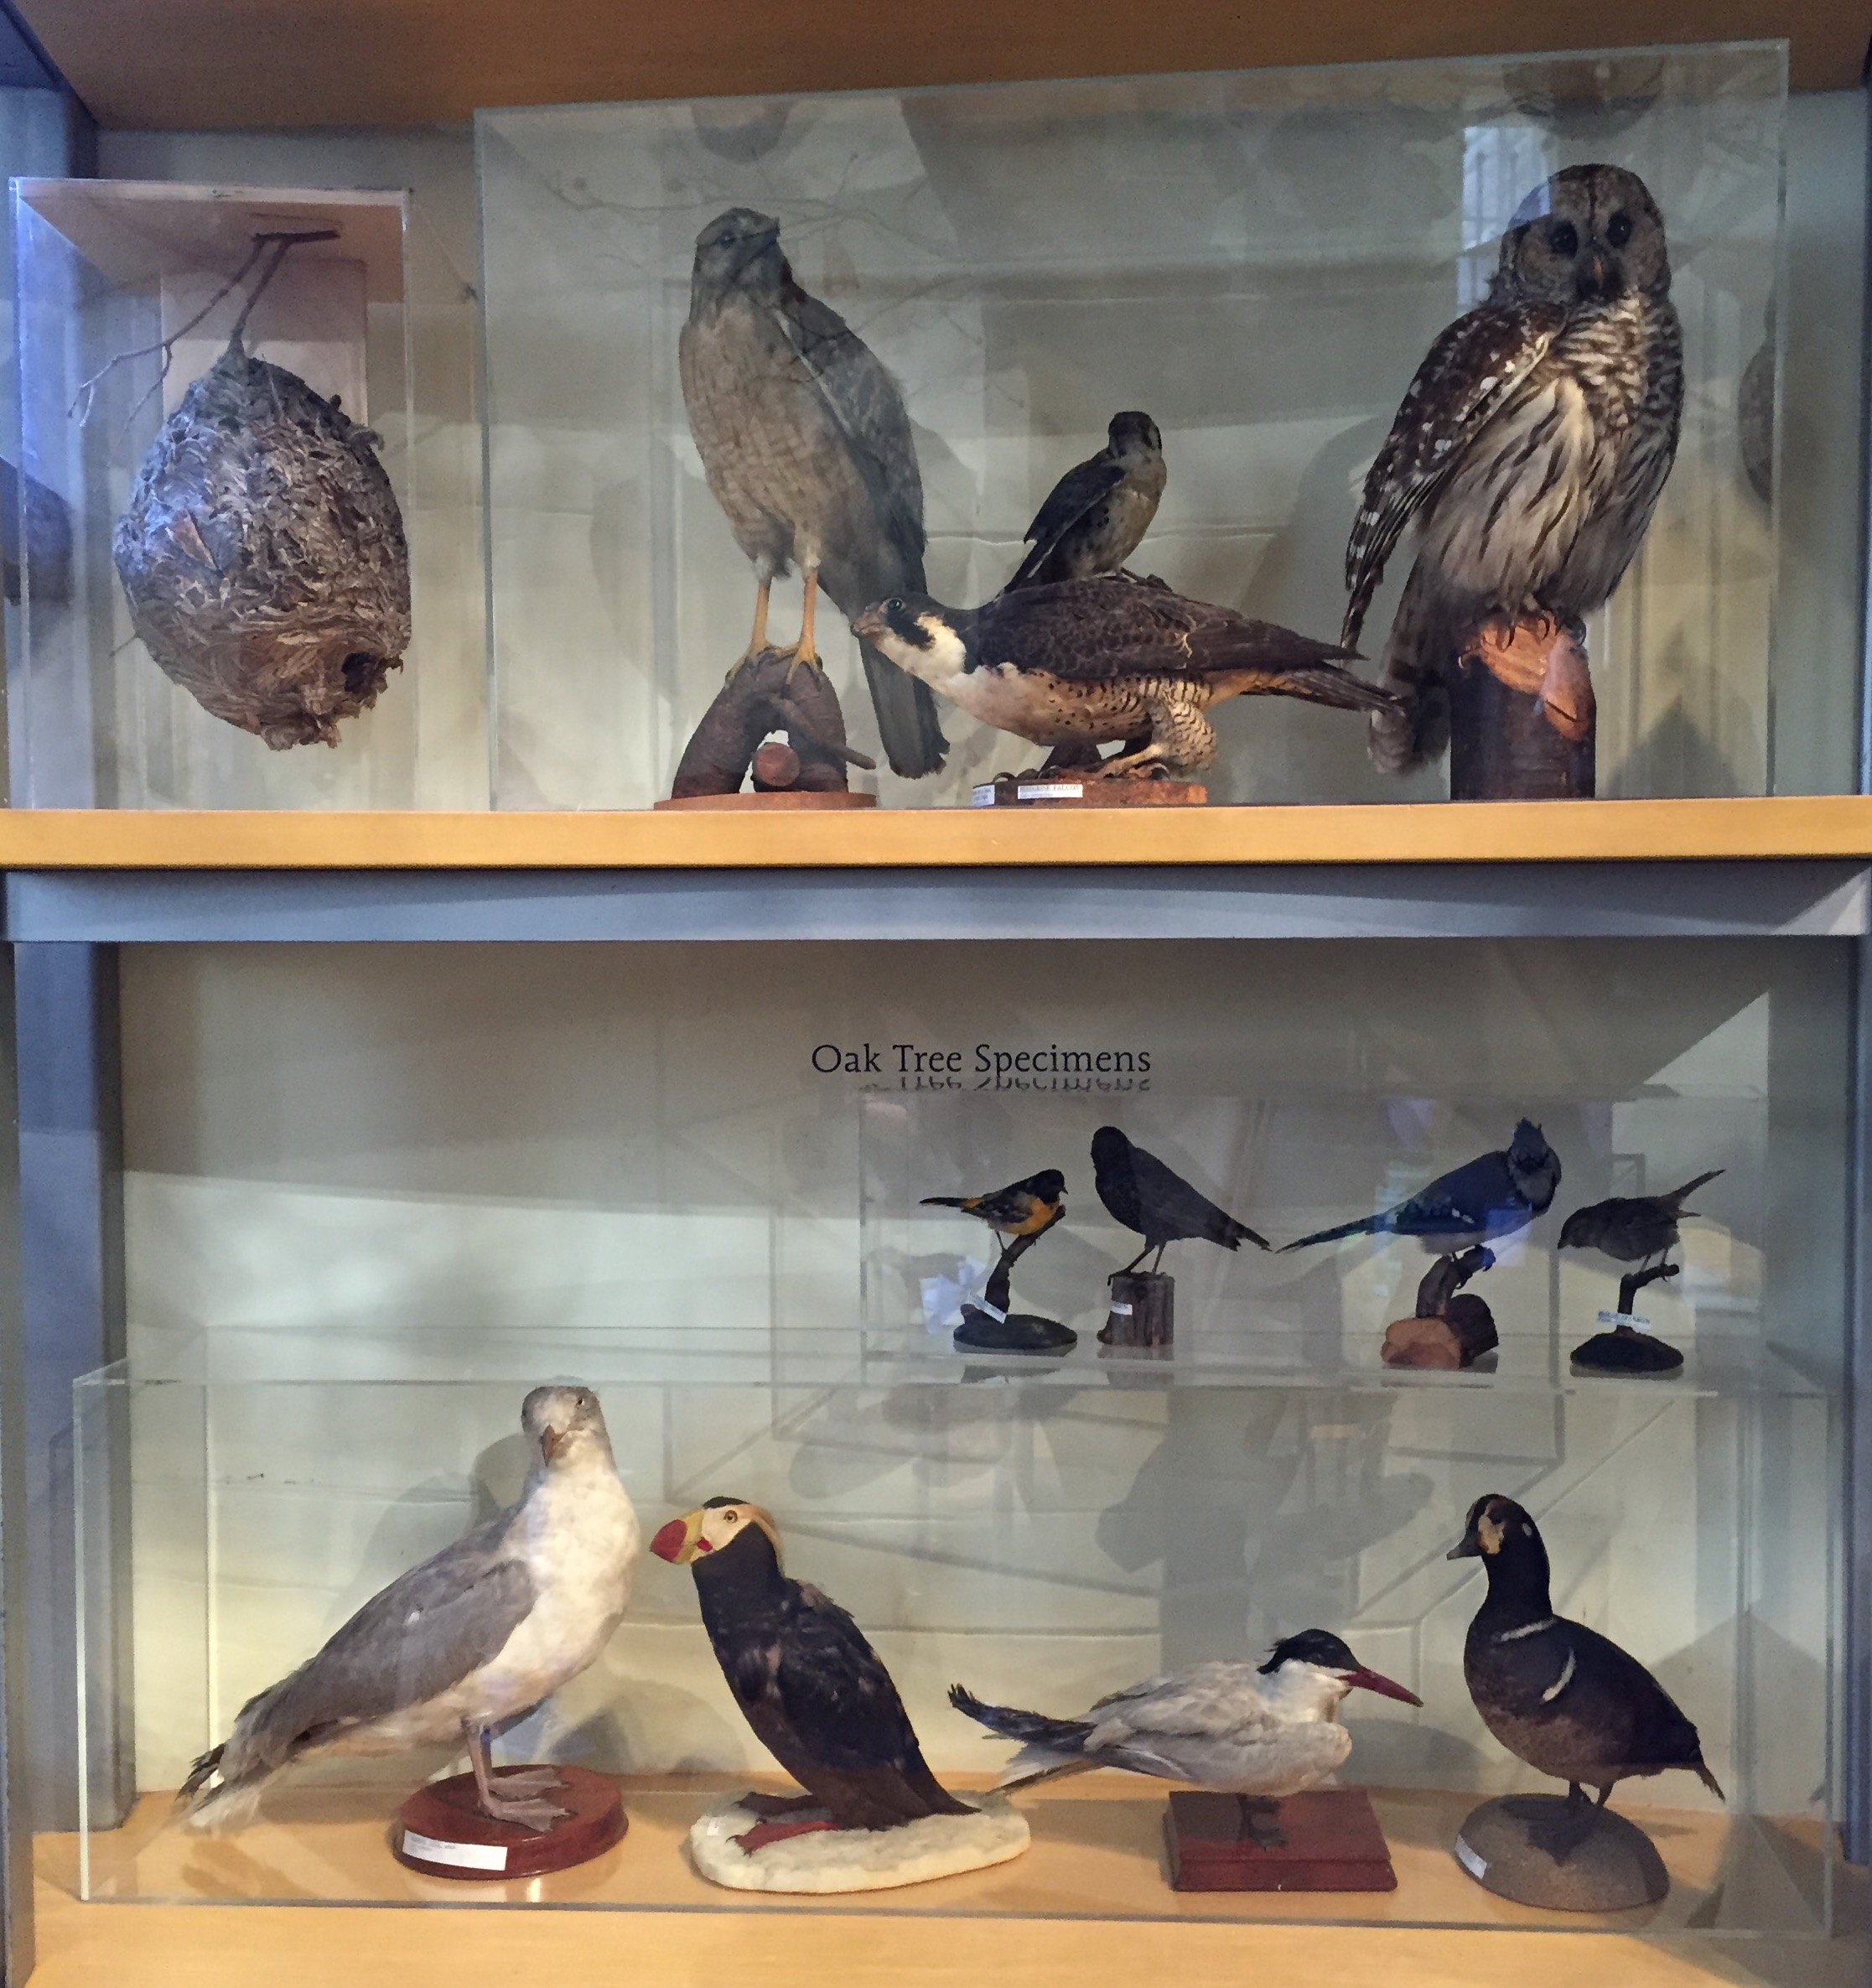
\includegraphics[width=0.48\textwidth]{figures/display_cases}
  \caption{The display cases in the American Museum of Natural History's Discovery Room, with the 12 bird specimens used in the intervention.} 
  \label{fig:display_cases}
\end{figure} 


\subsubsection{Procedure}

Children participated in the experiment during individual sessions with trained undergraduate research assistants in a corner of the AMNH Discovery Room. Participants were randomly assigned to one of three intervention conditions: Poster, Exhibit, or None.
Participants were first asked to list all of the birds they could name, as a means of establishing rapport. 
Second, they were asked to sort 24 bird cards (8 water birds, 8 raptors, and 8 songbirds) into piles ``that go together by nature.'' They were given three baskets, but were not explicitly told to form three piles--nor instructed to if they asked.
This sorting task offered a simple way of measuring their knowledge of the category structure, and was given a second time at the end of the experiment to measure changes in their representation of the category.
After each sort, participants were asked to describe each of the piles they made.

In addition to a control condition with no dialogue or visual intervention (None), there were two intervention conditions, using either a Poster (see Figure~\ref{fig:example_birds}) or an Exhibit of display cases (see Figure~\ref{fig:display_cases}) showing four birds from each cluster.  
In the intervention conditions, the experimenter showed the poster or display cases while giving a 2-minute dialogue that stressed the diversity of birds (e.g., color, size, and beak and talon shapes), while linking the distinguishing features of each cluster to their habitat and food sources (e.g., ``water birds swim in the water with webbed feet and eat fish'').

After the dialogue, children were given a series of 18 2-alternative forced choice induction sampling trials, an example of which is shown in Figure~\ref{fig:example_trial}.
Each trial offered two pairs of birds, and one bird was always shared across the two pairs (i.e., the harlequin duck in Figure~\ref{fig:example_trial}). Each trial always offered a same-cluster pair (e.g., two waterbirds) and a between-cluster pair (e.g., a waterbird and a raptor, as in Figure~\ref{fig:example_trial}).
Children were told they were scientists trying to determine whether all birds (on category induction trials) or all birds of a given type (e.g., all raptors; cluster induction trials) had some property (e.g., `podotheca'). They were asked to choose which pair of birds (left or right) they would like to test in order to make that determination.
The first 9 sampling trials had questions targeting induction to the entire bird category, of the form: ``You are a scientist who wants to find out if BIRDS have podotheca. Which set of birds do you want to look at to learn about BIRDS?''
Three of these category-induction trials were easy, in that the same-cluster pairs of birds were two exemplars of the same species (e.g., photos of two puffin exemplars). The other six were difficult, in that the same-cluster pair showed birds of different species (e.g., a duck and a puffin, in Figure~\ref{fig:example_trial}).
The final 9 sampling trials had questions targeting each cluster (3 per cluster), of the form: ``Here are two sets of birds. You are a scientist who wants to find out if RAPTORS have cancella. Which set of birds do you want to look at to learn about RAPTORS?''
For each cluster, one of the cluster-induction trials was easy (i.e., the same-cluster pair showed two birds of the same species), while the other two per cluster were difficult, with the same-cluster pair comprised of different species.

The same 12 exemplar birds were shown in the poster as in the exhibit, and were also represented among the 24 cards for sorting, and in the induction sampling trials.
Thus, a total of 24 bird species (8 per cluster) were introduced in the experiment, 12 of which were used in the interventions, and the remainder of which also appeared in both the pile sorting and sampling trials. 

\begin{figure}[h]
  \centering
  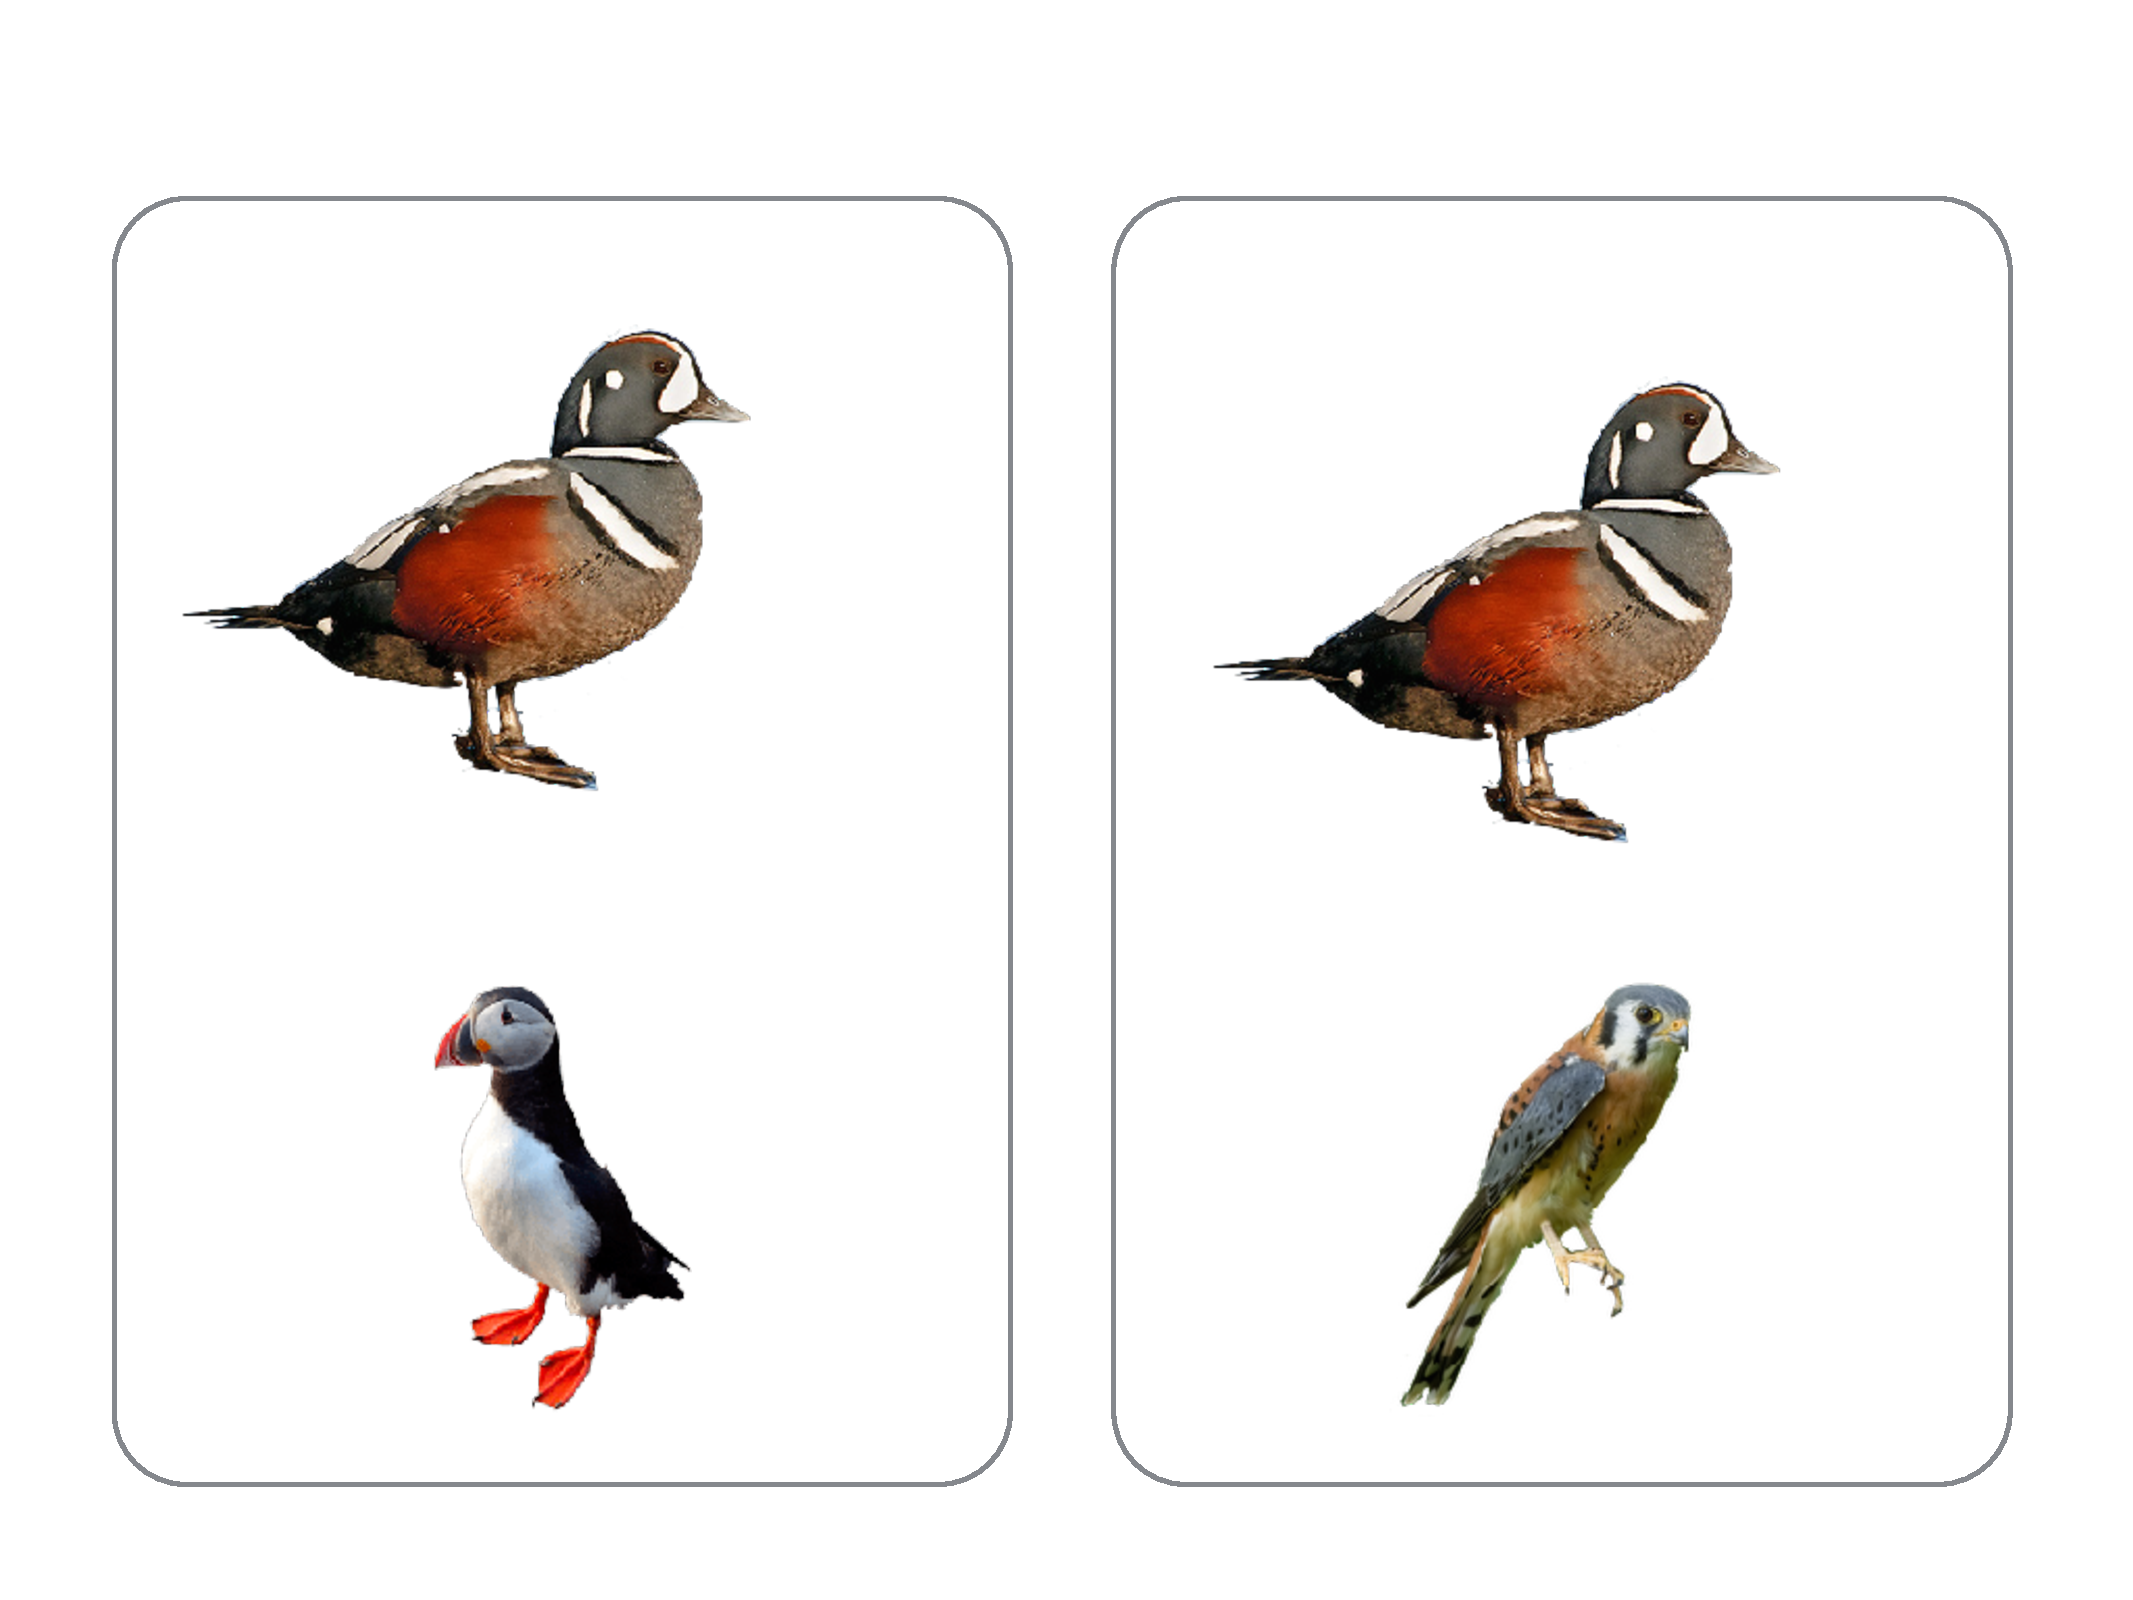
\includegraphics[width=0.4\textwidth]{figures/ex_trial}
  \caption{Example of a difficult induction sampling trial. Participants might be asked to choose which sample of birds (left pair or right pair) they would like to test to determine whether all birds (on category induction trials) or, e.g., all water birds (on cluster induction trials) have a property (e.g., `scutella'). For category induction, the right sample should be chosen for testing, as it is more diverse, containing a water bird and a raptor. For cluster (water bird) induction, the left sample should be chosen, as it contains two water birds (harlequin duck and puffin). On easy trials, one sample would contain two identical birds (e.g., two puffins). }
  \label{fig:example_trial}
\end{figure} 


\subsection{Results}
Results were analyzed for 259 participants: 94 in the Exhibit condition (24 aged-5, 26 aged-6, 20 aged-7, and 24 aged-8), 66 in the Poster condition (16 aged-5, 15 aged-6, 22 aged-7, 13 aged-8), and 99 in the None condition (23 aged-5, 32 aged-6, 24 aged-7, 20 aged-8).
Data from 8 other participants were eliminated due to failure to complete the experiment or experimenter error.


\subsubsection{Bird Sorts}

Participants' sorts of the 24 birds were first examined according to the descriptions that they gave their piles.
Experimenters sanitized and aggregated the pile sort descriptions, and attempted to assign a single label to the scheme by which each participant carried out their first (pre-intervention) and second (post-intervention) sorts.
Participants' aggregated pile sort explanations are shown in Table~\ref{tab:sorts}.
In some cases, participants gave no interpretable description (\emph{none}), or gave a \emph{mix} of features (e.g., color and size for one pile, habitat for another).
It is clear that many participants, both pre- and post-intervention, sorted according to a single salient dimension such as size (111 first sort; 67 second), a physical feature (24 first; 21 second) or color (20 first; 15 second).
However, cluster-based sorting is the only strategy that saw a marked increase from the first to the second sort (25 to 120 participants), with most single-dimension strategies seeing corresponding decreases (e.g., size: 111 to 67; habitat: 35 to 11).
In terms of their qualitative descriptions, participants have largely shifted from single-dimension sorting strategies to a cluster-based strategy. 
Next, we quantified the degree to which participants' sorts improve in each intervention condition with respect to the ground truth.

\begin{table}
\begin{center}
\begin{tabular}{ |c|c| } 
 \hline
 {\em Pre-Intervention Sort} & {\em Post-Intervention Sort}  \\ \hline
 size (111) & cluster (120)  \\ 
 habitat (35) & size (67)  \\      
 mix (27) & feature (21) \\
 cluster (25) & color (15) \\
 feature (24) & mix (12) \\
 color (20) & none (12) \\
 none (10) & habitat (11) \\
 \hline
 252  & 258  \\  
 \hline
\end{tabular}
\end{center}
\caption{Categories of participants' pile sort explanations.}
    \label{tab:sorts}
\end{table}

To measure the quality of participants' sorts, we compared the piles from each participant's first and second sorts to the objectively correct cluster sort (three piles: 8 raptors, 8 songbirds, and 8 waterbirds). 
The similarity between a participant's sort and the correct cluster sort was measured with the adjusted Rand Index \cite{Rand:1971}, which counts the number of pairs of elements in $S$ (the cards) that are in the same subset in partition $X$ (a participant's piles) and in the same subset in $Y$ (the 3-pile objective), as well as the number of pairs of elements in $S$ that are in different subsets in $X$ and that are in different subsets in $Y$.
These agreements between sort $X$ and sort $Y$ are divided by the number of all possible pairs (agreements + disagreements), and thus the Rand index is 0 when two sorts do not agree on any pair of cards, and 1 when sorts are exactly the same.
The adjusted Rand Index corrects for chance using the expected similarity of all pair-wise comparisons between clusterings specified by a random model, and can thus on occasion have negative values if the index is less than expected by chance \cite{Hubert:1985}.

\begin{figure}[h]
  \centering
  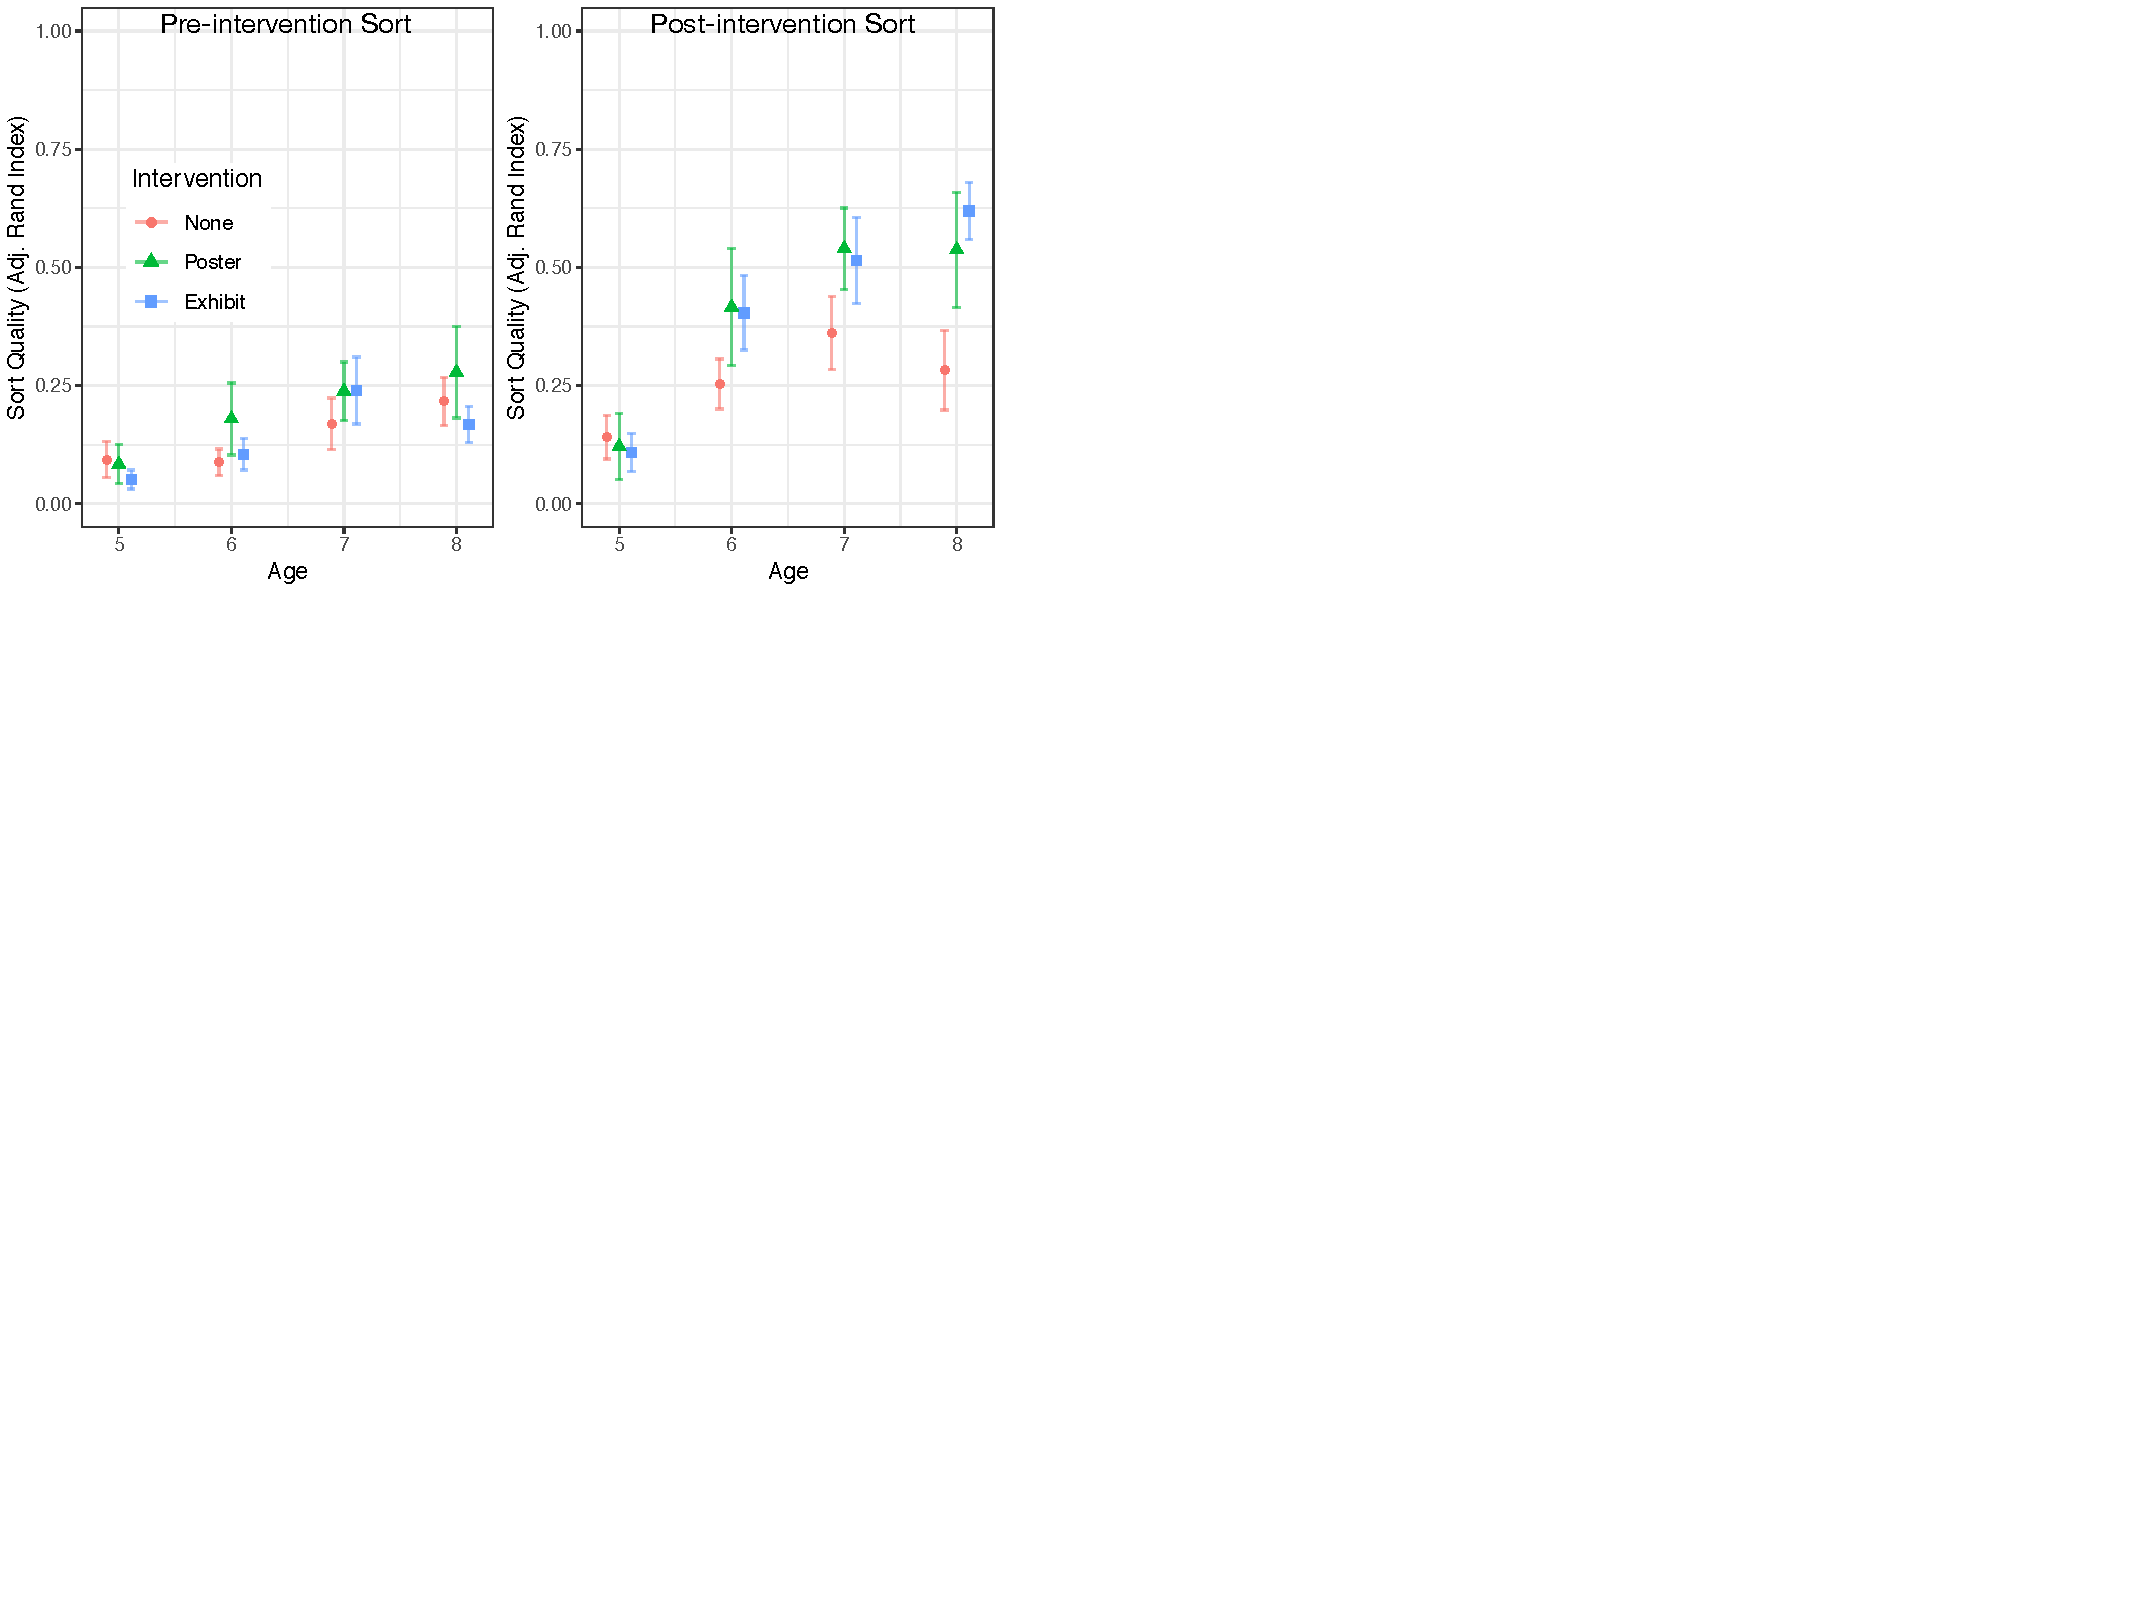
\includegraphics[width=0.48\textwidth]{figures/sort1_sort2_combined}
  \caption{Mean pre-intervention sort quality (left panel) and post-intervention sort quality (right panel) by age and intervention condition. Error bars show +/-1SE.}
  \label{fig:sort-quality}
\end{figure} 

The adjusted Rand Index of participants' sorts and the correct clustering (i.e., sort quality) were subjected to a repeated measures ANCOVA with sort time (pre-/post-intervention) as the repeated measure, age (5.00-8.93 years) as covariate, and intervention condition (poster, exhibit, or none) as a between-subjects factor.
Sort quality improved more across time in the intervention conditions (from pre- to post-intervention) than in the control condition (as evidenced by an interaction of intervention and sort (F(2,253)=4.45, $p=.01$); there were also subsumed main effects of sort time (pre- to post-intervention F(1,253)=97.42, $p<.001$) and intervention condition (F(2,253)=3.49, $p=0.03$). 
Participants in the two intervention conditions showing more improvement in sort quality over time ($M=.25$) than participants receiving no intervention (Welch's t(245.7)=2.93, $p=0.004$). 
Sort quality also improved across time more for older children than younger children (interaction of age and sort (F(1,253)=13.75, $p<.001$), with a subsumed main effect of age (F(1,253)=35.22, $p<.001$).
Figure~\ref{fig:sort-quality} shows participants' mean sort quality on the pre- (first; left panel) and post-intervention (second; right panel) sorts by age and condition.
Having shown that the interventions helped improve children's understanding of the clustered structure of the bird category, we turned to the induction sampling choices to determine if diversity-based reasoning also improved, using the quality of their second sort as a covariate.



\subsubsection{Induction Sampling Choices}

We separately analyze the sampling trials that were targeted at inducing to a specific cluster, and the sampling trials that were targeted at inducing to the entire category. 
On the cluster induction trials, participants should choose the pair of birds from the targeted cluster, rather than the diverse pair. 
In contrast, on the category induction trials, participants should choose the diverse pair, with birds representing two different clusters.
Thus, to analyze the cluster induction trials, participants' binomial choices for each trial (0=choosing the diverse pair, 1=choosing the cluster pair) were subjected to a logistic mixed-effects regression with intervention condition as a between-subjects factor and trial difficulty (easy or difficult) as a within-subjects factor, and age and quality of second sort as covariates\footnote{Covariates scaled and zero-centered.}.

On the cluster trials, there was no significant main effect of intervention (F(2,243.5)=0.70, $p=.50$), nor any significant interactive effects involving intervention, as shown in Figure~\ref{fig:sampling-choice} (left).
Children were more likely to select samples containing only members of the cluster that they were trying to learn about (the more informative samples in this case) with age, (F(1,244.2)=20.39, $p<.001$), and they were also more likely to do so if they had more accurate representations of the category structure as indicated by their post-intervention category sort (F(1,246.1)=27.15, $p<.001$). 
There was a significant interaction of age and second sort quality (F(1,241.5)=5.57, $p=.02$).
Shown in Figure~\ref{fig:induction-age-by-sort}, children with high-quality (4th quartile: ARI$>.65$) second sorts are near-ceiling at correctly choosing the within-cluster sample for induction--even the 5- and 6-year-olds.
The cluster pair was chosen significantly less often on difficult trials ($M=0.69$) than on easy trials ($M=0.77$, F(1,255.2)=19.05, $p<.001$).
All other effects were not significant. 

\begin{figure}[ht]
  \centering
  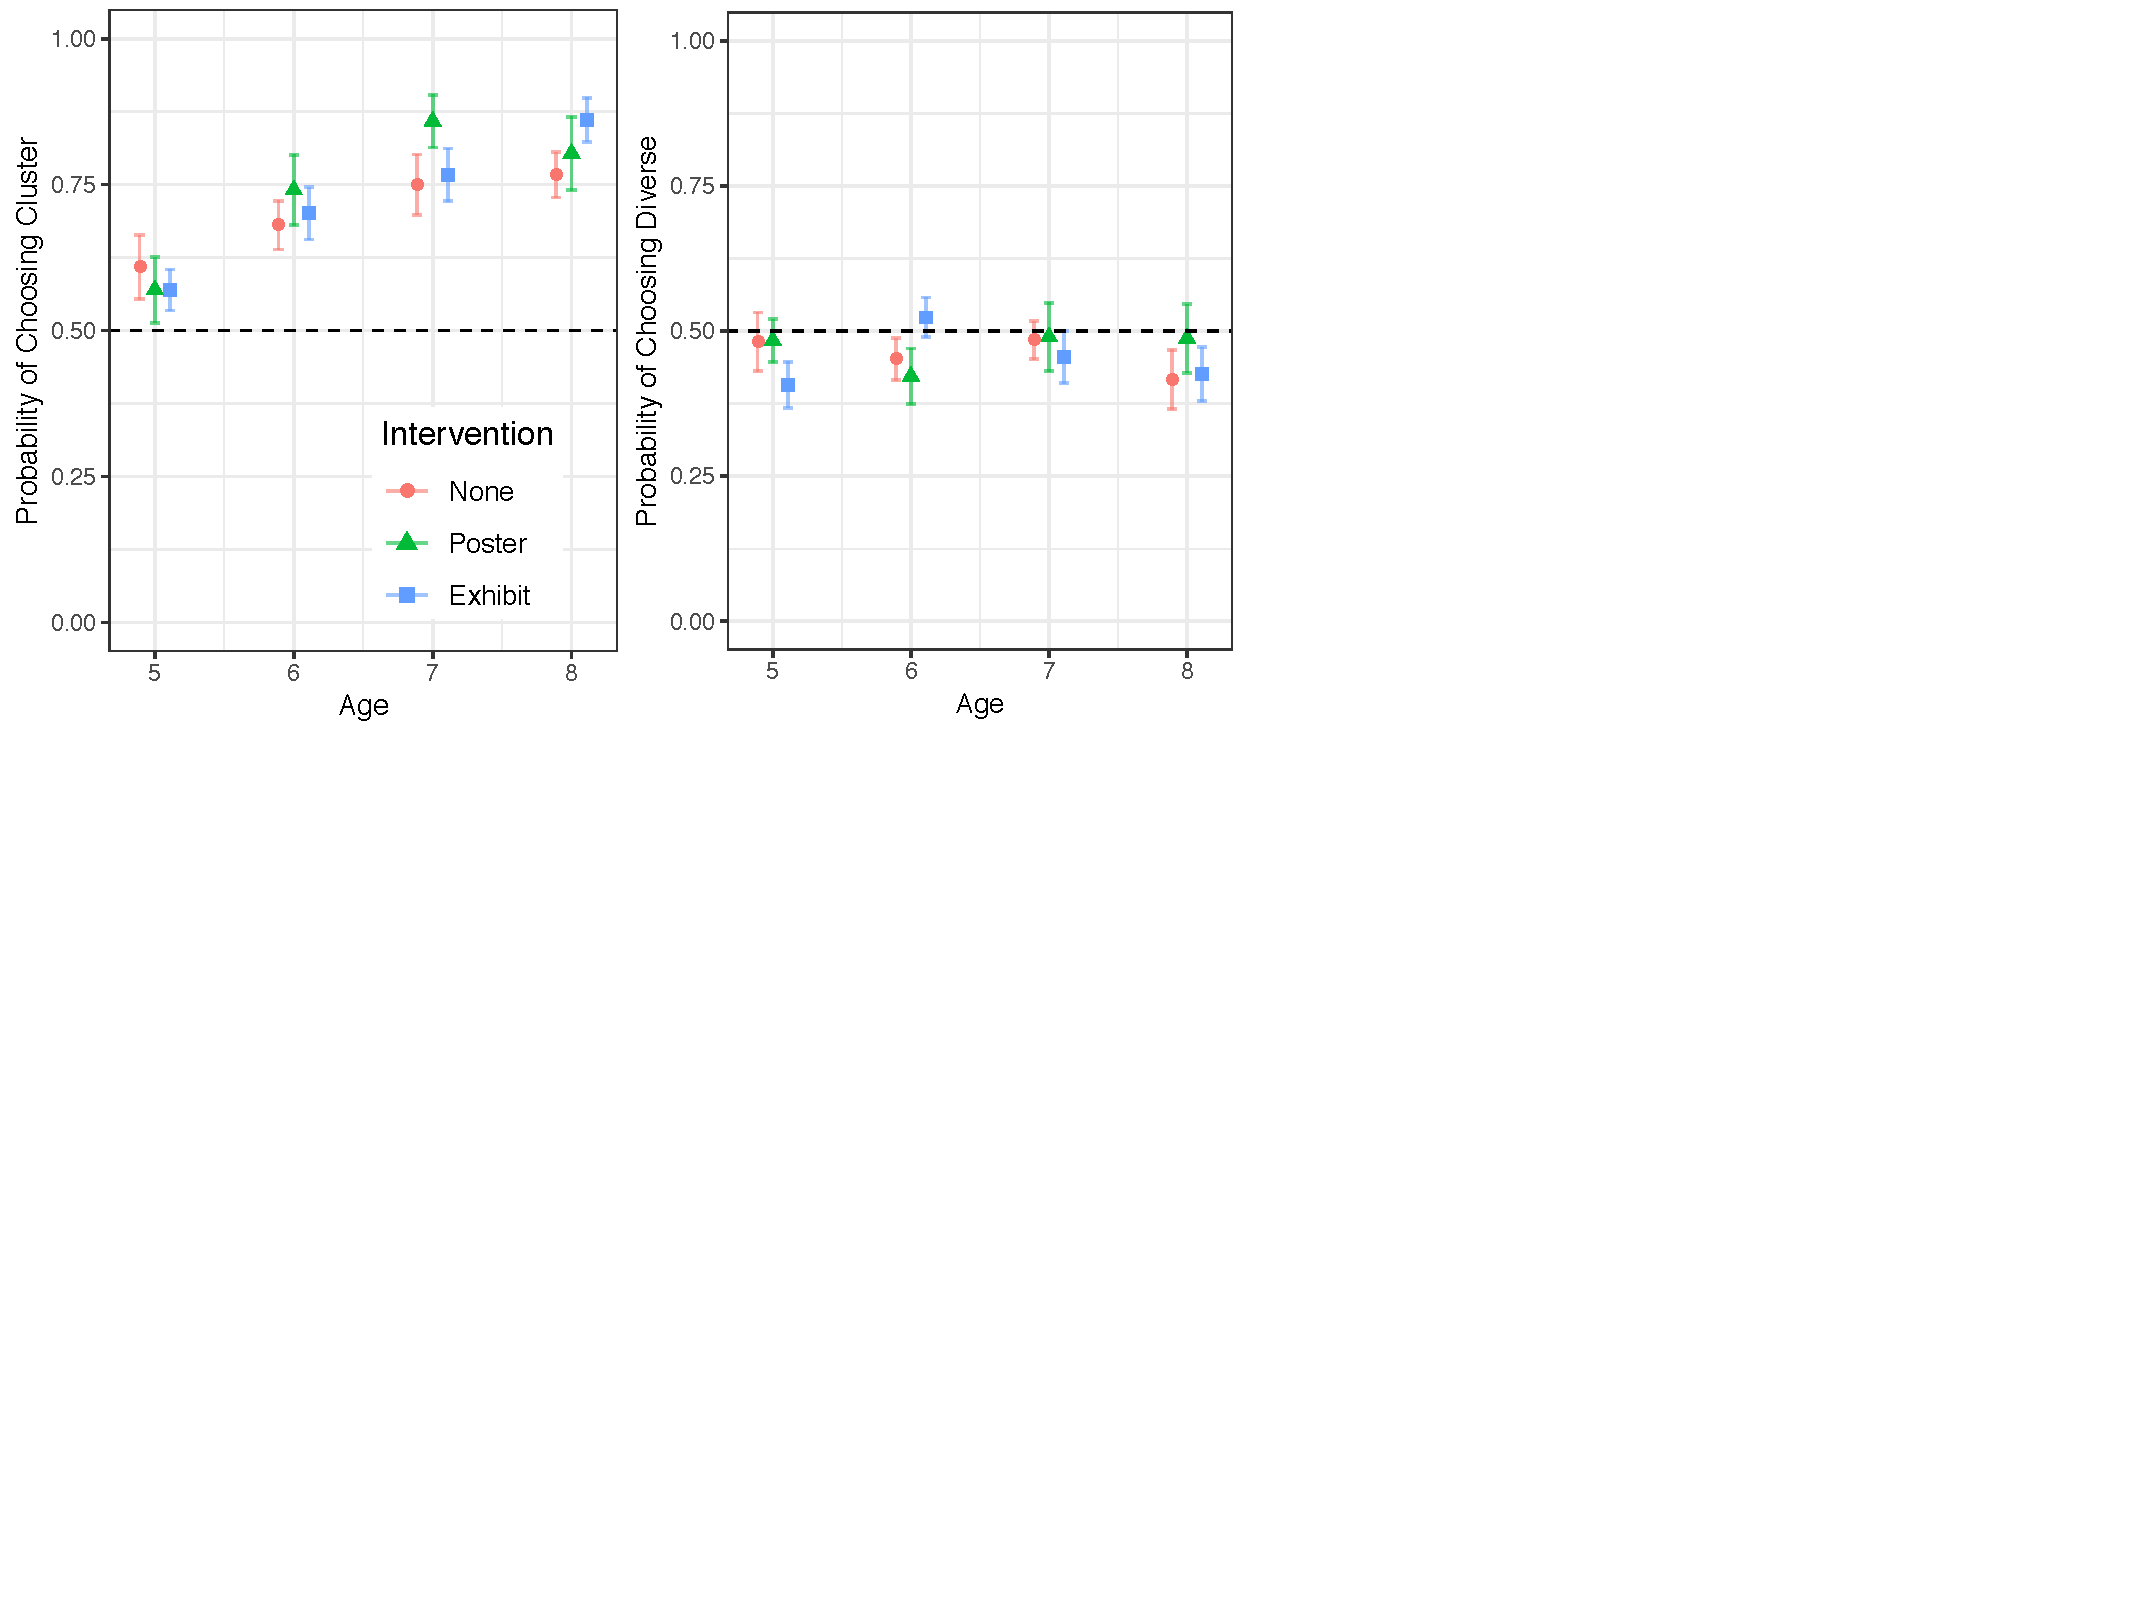
\includegraphics[width=0.48\textwidth]{figures/induction_sampling_choices_combo}
  \caption{Mean proportion of correct sampling choice--nondiverse for cluster induction (left), and diverse for category induction (right)--by age group and intervention condition. Error bars show +/-1SE, and dotted lines show chance.}
  \label{fig:sampling-choice}
\end{figure} 
\vspace{-.1cm}
\begin{figure}[ht]
  \centering
  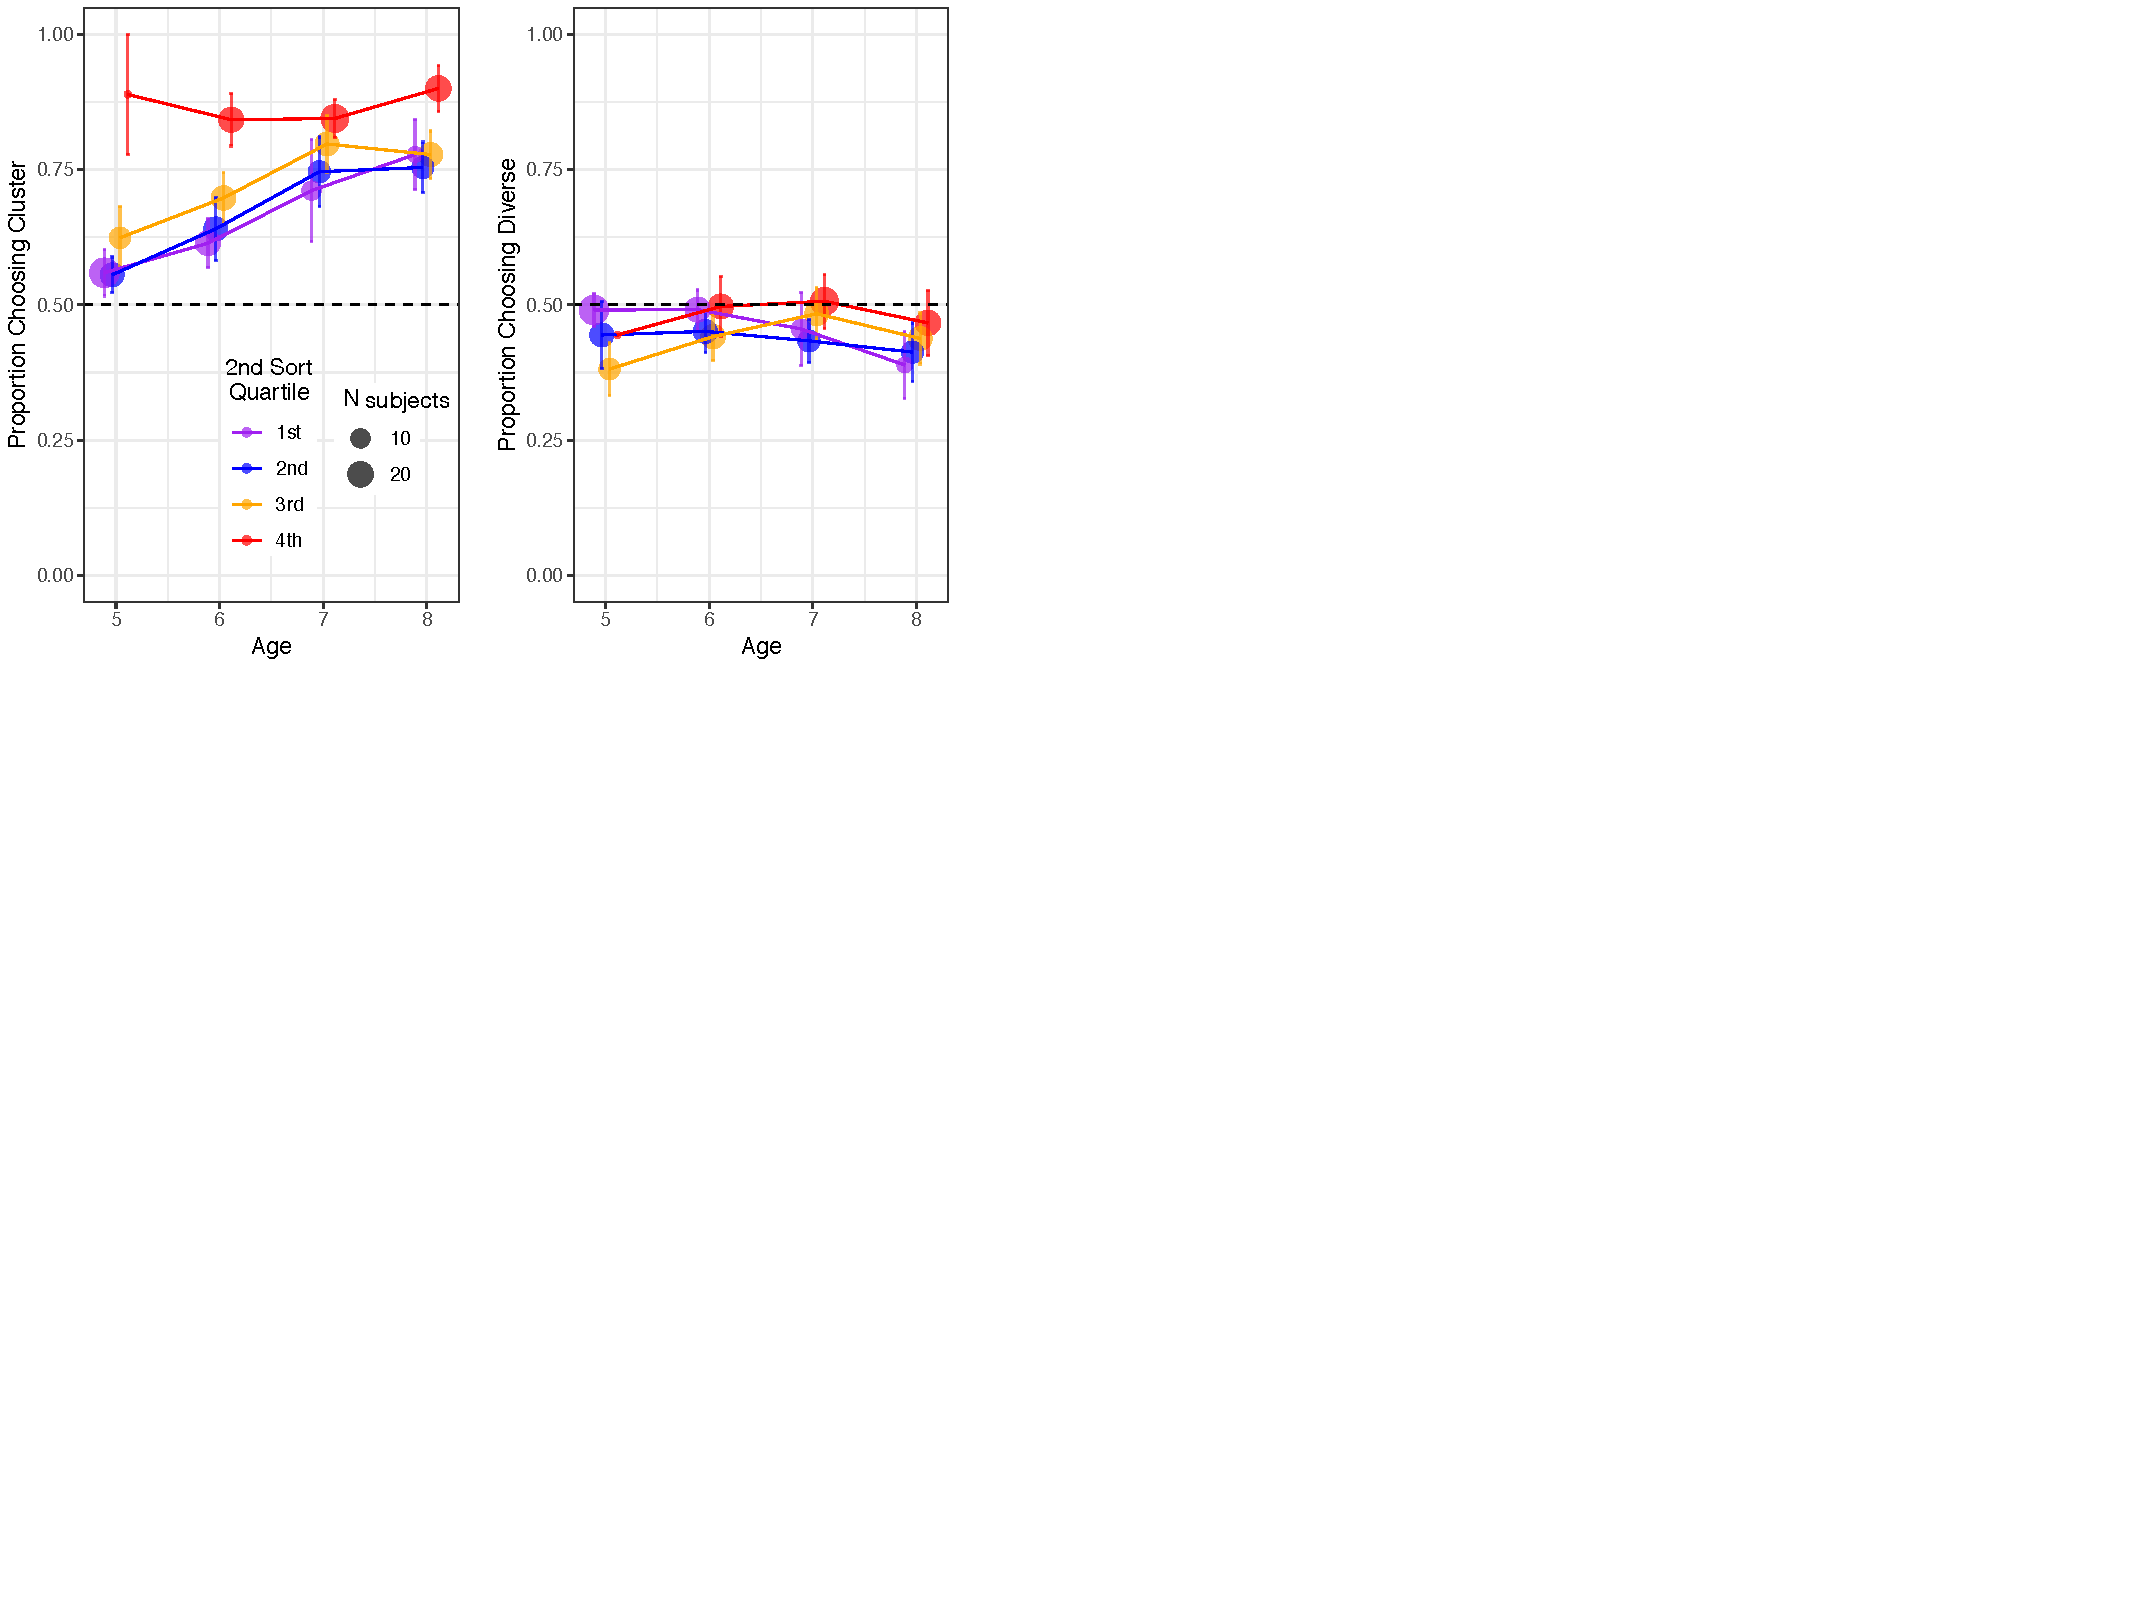
\includegraphics[width=0.48\textwidth]{figures/induction_sampling_age_by_sort2}
  \caption{Mean proportion of correct sampling choice for induction (left: nondiverse for cluster, right: diverse for category) as a function of age and quartile of 2nd sort's quality. Error bars show +/-1SE, and dotted lines show chance.}
  \label{fig:induction-age-by-sort}
\end{figure} 
\vspace{-.1cm}
To analyze the category induction trials, participants' binomial choices for each trial (0=choosing the non-diverse pair, 1=choosing the diverse pair) were subjected to a logistic mixed-effects regression with intervention condition as a between-subjects factor and trial difficulty (easy or difficult) as a within-subjects factor, age and second sort quality, scaled and centered, as covariates.
As seen in Figure~\ref{fig:sampling-choice} (right), there was no significant main effect of intervention (F(2,266.0)=0.08, $p=.93$), nor any significant interactive effects involving intervention: participants of all ages were near-chance at correctly choosing the diverse pair (F(1,267.1)=0.00, $p=.98$).
There was no significant main effect of second sort quality (F(1,269.6)=0.02, $p=.88$).
Easy trials had marginally higher performance than difficult trials (F(1,1384.6)=3.67, $p=.06$). 
There was once again a significant interaction of age and second sort quality (F(1,262.8)=5.61, $p=.02$), shown in Figure~\ref{fig:induction-age-by-sort} (right).
Children with 4th quartile post-intervention sorts were picking the diverse pair at close to chance rates at all ages, while 8-year-olds  with lower-quality sorts preferred the less informative, nondiverse samples. 
All other effects were not significant. 


Given that participants were at best choosing the diverse sample at as often as expected by chance on category induction trials, we investigated whether they showed any systematic sampling strategies on these items. 
As a reminder, each sampling trial presented three birds: one appearing in both samples, one from the same cluster, and one from a different cluster. 
We considered the possibility that, among the two varying birds per trial, children preferred to sample some types (i.e. clusters) of birds over others.
Table~\ref{tab:choices} shows, for each type of sampling trial (category vs. each cluster), the proportion of trials on which participants chose a sample containing a bird of a given cluster.
For category induction trials, participants avoided choosing samples with waterbirds, choosing them only 21\% of the time, significantly different than the 40\% raptors and 39\% songbirds chosen ($\chi^2(2, N=2,373) = 162.7$, $p<.001$).
Indeed, this bias against sampling waterbirds extended to the cluster induction trials: participants had lower rates of choosing a waterbird to induce to all waterbirds (48\%) than of choosing a raptor to induce to all raptors (80\%), or than choosing a songbird to induce to all songbirds (71\%).
For incorrect answers, waterbird was the least popular choice (0\% for songbird trials and 8\% for raptor trials).
It may be that participants avoid waterbirds because it is the cluster that they find least typical of birds. 
To verify this, we asked 13 adults to rate the typicality (1-7; 1=atypical, 7=very typical) of the 8 waterbirds, 8 raptors, and 8 songbirds used in this experiment. 
They were shown the same unlabeled pictures as children saw, in a randomized order. 
On average, participants found songbirds the most typical ($M=5.92$), followed by raptors ($M=4.41$), and waterbirds ($M=3.54$).

\begin{table}
\begin{center}
\begin{tabular}{ c|ccc } 
 \hline
          &  & {\em Chosen: }  & \\
{\em Induce To:} & Raptor & Songbird & Waterbird \\ \hline
All Birds &  0.40  &  0.39   &  0.21 \\ \hline
Raptors   &  0.80  &  0.13   &  0.08 \\
Songbirds &  0.29  &  0.71   &  0.00 \\
Waterbirds & 0.36  &  0.16   &  0.48 \\
 \hline
\end{tabular}
\end{center}
\caption{Participant's choices on induction trials.}
    \label{tab:choices}
\end{table}
\vspace{-.15cm}


\section{General Discussion}
\vspace{-.1cm}
The present study investigated whether teaching children about the clustered structure of the bird category would increase the diversity of their sampling choices in a category induction task.
The didactic dialogue and intervention displays significantly shifted children's representation of the bird category, as evidenced by a shift from them sorting birds into piles according to single dimensions (e.g., size or color), to them predominantly sorting by cluster (songbird, waterbird, and raptor) after the intervention.
Moreover, children's pile sorts post-intervention were much closer to the actual cluster structure, as measured by adjusted Rand index.
Despite this shift in children's representation of the bird category, we found no evidence that either intervention display improved their category induction sampling choices. Children of all ages were near-chance at choosing the diverse sample when inducing to the category. Yet, the quality of children category's representations was indeed related to their sampling behavior in some cases. Younger children with more accurate category representations chose more informative samples on the cluster-induction trials. Also, older children with more accurate category representations chose diverse samples more often than their age-matched peers with less accurate category representations, although even these children did not choose diverse samples more often than expected by chance. 

Given that the intervention conditions increased the accuracy of children's category representations, and category representations were somewhat related to children's sampling decisions, it is surprising that the intervention was not powerful enough to increase the efficiency of children's sampling strategies. One possibility is that children simply apply a different standard for evaluating the informativeness of samples. For instance, Foster-Hanson et al. (2019) found that young children prefer to examine highly prototypical examples instead of samples that cover variation. This tendency might have been behind children's decisions in the present study to avoid sampling waterbirds--the least typical birds presented according to adult raters. From this perspective, although the intervention made children more aware of the structured variability that exists within the category, perhaps it did not lead them to view that variation as informative because they prefer to rely on separate criteria (typicality) for evaluating samples of evidence.  


We conclude that it is unlikely that simply knowing the clustered structure of a natural category is sufficient for children to realize the inductive power of choosing diverse samples.
There is certainly merit to learning the structure of natural categories beyond any benefit to diversity-based reasoning, but
future interventions seeking to increase appreciation for diverse sampling strategies may wish to demonstrate to children the value of choosing diverse samples more directly.


\subsection{Acknowledgments}

This work was supported by the John Templeton Foundation ``Varieties of Understanding'' grant to T.M.G. and M.R., National Science Foundation grant BCS-1255538 to T.M.G., and National Science Foundation grant BCS 1729540 to M.R.
We are grateful to Kathryn Yee, Aja Blanco, Christina Chu, and Talena Smith for data collection, and to Daniel Zeiger and the staff of the American Museum of Natural History's Discovery Room for their support of this project.

\bibliographystyle{apacite}


\setlength{\bibleftmargin}{.125in}
\setlength{\bibindent}{-\bibleftmargin}
\vspace{-0.1cm}
\bibliography{clusters_refs}

\end{document}
